% ------------------------------------------------------------------------------
% TYPO3 CMS 6.2 LTS - What's New - Chapter "Install Tool" (Serbian Version)
%
% @author	Sinisa Mitrovic <mitrovic.sinisaa@gmail.com>
% @license	Creative Commons BY-NC-SA 3.0
% @link		http://typo3.org/download/release-notes/whats-new/
% @language	Serbian
% ------------------------------------------------------------------------------
% Chapter: Install Tool
% ------------------------------------------------------------------------------

\section{Install Tool}
\begin{frame}[fragile]
	\frametitle{Install Tool}

	\begin{center}\huge{Poglavlje 1:}\end{center}
	\begin{center}\huge{\color{typo3darkgrey}\textbf{Install Tool}}\end{center}

\end{frame}

% ------------------------------------------------------------------------------
% Installation
% ------------------------------------------------------------------------------

\begin{frame}[fragile]
	\frametitle{Install Tool}
	\framesubtitle{Instalacija}

	\begin{itemize}
		\item Samo \underline{jedan} paket je potreban za instalaciju:\newline
				\texttt{typo3\_src-6.2.x.tar.gz} (velicinie fajla oko 20MB)
		\item "Dummy" i  "Blank" paketi zastareli su
		\item Instalacija:
			\begin{itemize}
				\item Raspakovati arhivu u koren sajta
				\item Mapraviti symbolic link-ove kao sto je trazeno
				\item U pretrazivacu uneti adresu sajta
				\item TYPO3 Installer pokrece 1-2-3-4-koraka carobnjaka
			\end{itemize}

	\end{itemize}

\end{frame}

% ------------------------------------------------------------------------------
% Installation
% ------------------------------------------------------------------------------

\begin{frame}[fragile]

	\frametitle{Install Tool}
	\framesubtitle{Instalacija}

	\begin{itemize}
		\item Obezbedjuje da su svi potrebni fajlovi I direktorijumi na svom mestu
		\item Fajlovi potrebni za dodatna podesavanja bice kreirani automatski
		\item Sledeci symbolic link-ovi \underline{moraju} da postoje:

		\begin{itemize}
			\item \texttt{typo3\_src}	\tabto{2cm} (upucuje na TYPO3 izvorni direktorijum)
			\item \texttt{typo3}		\tabto{2cm} (upucuje na direktorijum: \texttt{typo3\_src/typo3})
			\item \texttt{index.php}	\tabto{2cm} (upucuje na fajl: \texttt{typo3\_src/index.php})
		\end{itemize}

		\item Nema dodatnih fajlova/direktorijuma koji su neophodni za instalaciju Typo3
		\item Direktorijum \texttt{t3lib} je uklonjen
		\item Dodatni detalji: Typo3 instalacija i uputstvo za unapredjenje:\newline
			\url{http://docs.typo3.org/typo3cms/InstallationGuide}

	\end{itemize}

\end{frame}

% ------------------------------------------------------------------------------
% Re-Development
% ------------------------------------------------------------------------------

\begin{frame}[fragile]
	\frametitle{Install Tool}
	\framesubtitle{Reprogramiranje}

	\begin{columns}[T]

		\begin{column}{.5\textwidth}
			\begin{itemize}
				\item Reprogramiran od pocetka koriscenjem Fluid-a
				\item \underline{Prvi} korak testira sistemsko okruzenje i javlja probleme
				\item Prijavljeni problemi mogu biti ispravljeni\newline (i ponovo testirani) ili zanemareni
				\item Pogresno podesavanje core-a (na primer nema preporucenih symbolic link-ova) se takodje prijavljuje kao problem
			\end{itemize}
		\end{column}

		\begin{column}{.5\textwidth}
			\begin{figure}\vspace*{-0.4cm}
				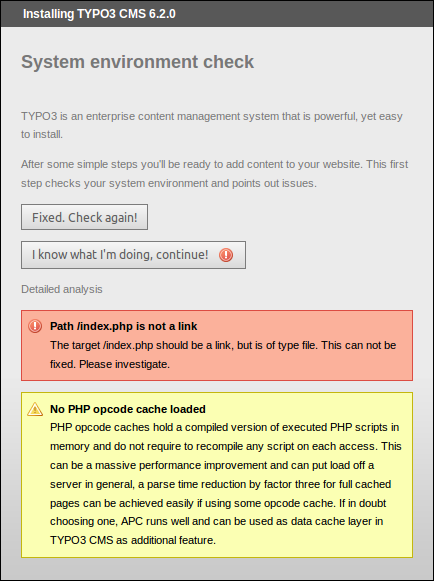
\includegraphics[width=0.8\linewidth]{Images/InstallTool/SystemEnvironmentCheck.png}
			\end{figure}
		\end{column}

	\end{columns}

\end{frame}

% ------------------------------------------------------------------------------
% Re-Development
% ------------------------------------------------------------------------------

\begin{frame}[fragile]
	\frametitle{Install Tool}
	\framesubtitle{Reprogramiranje}

	\begin{columns}[T]

		\begin{column}{.5\textwidth}
			\begin{itemize}
				\item \underline{Drugi} korak omogucuje korisnicima da unesu podatke za pristup bazi podataka
				\item Mozete izabrati tip veze
					\begin{itemize}
						\item Veza bazirana na TCP/IP
						\item Veza bazirana na Socket-u
					\end{itemize}
				\item Moguce su i alternative za MySQL
			\end{itemize}
		\end{column}

		\begin{column}{.5\textwidth}
			\begin{figure}\vspace*{-0.4cm}
				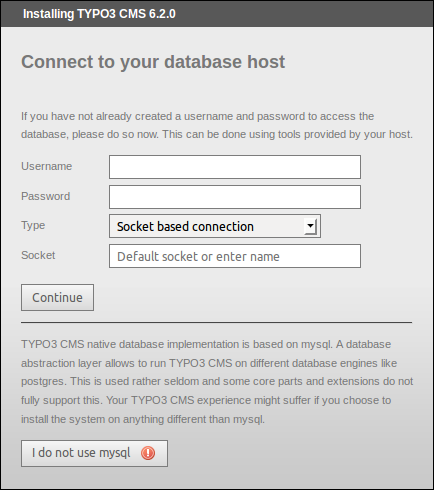
\includegraphics[width=0.8\linewidth]{Images/InstallTool/DatabaseConnectionDetails.png}
			\end{figure}
		\end{column}

	\end{columns}

\end{frame}

% ------------------------------------------------------------------------------
% Re-Development
% ------------------------------------------------------------------------------

\begin{frame}[fragile]
	\frametitle{Install Tool}
	\framesubtitle{Reprogramiranje}

	\begin{columns}[T]

		\begin{column}{.5\textwidth}
			\begin{itemize}
				\item \underline{Treci} korak omogucava korisniku da izabere/kreira bazu podataka\newline
					(kao i kod TYPO3 < 6.2)
				\item \underline{Cetvrti} korak omogucava korisniku da postavi lozinku za admin korisnika\newline (koja je takodje pocetna lozinka za Install Tool) i ime sajta
			\end{itemize}
		\end{column}

		\begin{column}{.5\textwidth}
			\begin{figure}\vspace*{-0.4cm}
				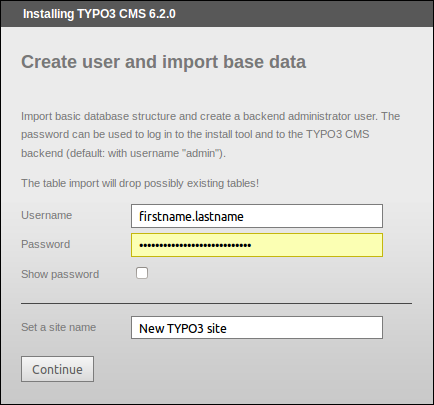
\includegraphics[width=0.8\linewidth]{Images/InstallTool/AdminPasswordAndSiteName.png}
			\end{figure}
		\end{column}

	\end{columns}

\end{frame}

% ------------------------------------------------------------------------------
% Clear All Cache
% ------------------------------------------------------------------------------

\begin{frame}[fragile]
	\frametitle{Install Tool}
	\framesubtitle{Brisanje kompletnog kesa}

	\begin{itemize}
		\item Nova funkcija pod "Important actions" omogucava korisniku da izbrise kompletan kes.
		\item Ovo takodje radi ako kes sadrzi nevazeci PHP kod.\newline
			(koji moze da blokira TYPO3 CMS)
		\item Install Tool-u se moze pristupiti i direktno, zaobilazenjem TYPO3 instalacije koja ne funkcionise: \texttt{http://example.com/typo3/install}
	\end{itemize}

	\begin{columns}[T]
		\begin{column}{.3\textwidth}
			\begin{figure}\vspace*{-0.4cm}
				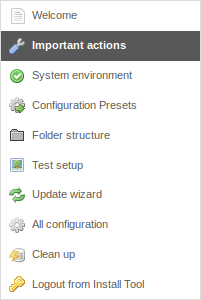
\includegraphics[width=0.7\linewidth]{Images/InstallTool/ImportantActions.png}
			\end{figure}
		\end{column}
		\begin{column}{.7\textwidth}
			\begin{figure}\vspace*{-0.4cm}
				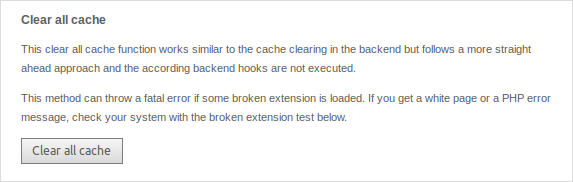
\includegraphics[width=0.9\linewidth]{Images/InstallTool/ClearAllCache.png}
			\end{figure}
		\end{column}
	\end{columns}

\end{frame}

% ------------------------------------------------------------------------------
% Clear All Cache
% ------------------------------------------------------------------------------

\begin{frame}[fragile]
	\frametitle{Install Tool}
	\framesubtitle{Clear All Cache}

	Redosled radnji prilikom izvrsenja "Clear all cache":

	\begin{enumerate}
		\item Sadrzaj direktorijuma \texttt{typo3temp/Cache} je izbrisan
		\item Tabele u bazi podataka \texttt{cf\_*} se prazne
		\item Fajlovi \texttt{ext\_localconf.php} i \texttt{ext\_tables.php}\newline
			se ucitavaju iz prosirenja
		\item \texttt{flushCaches()} se izvrsava
	\end{enumerate}

\end{frame}

% ------------------------------------------------------------------------------
% Check For Broken Extensions
% ------------------------------------------------------------------------------

\begin{frame}[fragile]
	\frametitle{Install Tool}
	\framesubtitle{Provera prosirenja koja ne rade}

	\begin{itemize}
		\item Nova funkcija u "Important actions" omogucava korisniku da proveri\newline
			da li prosirenje moze da se ucita, a da ne srusi sistem
		\item Veoma korisno prilikom unapredjenja sa TYPO3 4.5 na 6.2
	\end{itemize}

	\begin{columns}[T]
		\begin{column}{.3\textwidth}
			\begin{figure}\vspace*{-0.4cm}
				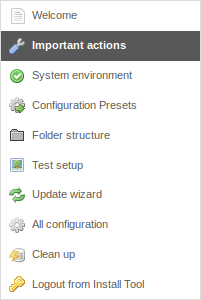
\includegraphics[width=0.7\linewidth]{Images/InstallTool/ImportantActions.png}
			\end{figure}
		\end{column}
		\begin{column}{.7\textwidth}
			\begin{figure}\vspace*{-0.4cm}
				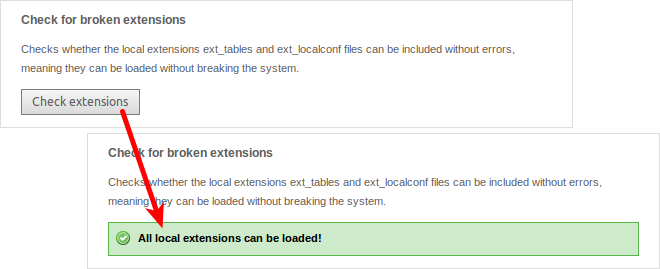
\includegraphics[width=1\linewidth]{Images/InstallTool/CheckForBrokenExtensions.png}
			\end{figure}
		\end{column}
	\end{columns}

\end{frame}

% ------------------------------------------------------------------------------
% Increased Security: Salted Passwords
% ------------------------------------------------------------------------------

\begin{frame}[fragile]
	\frametitle{Install Tool}
	\framesubtitle{Salted lozinke}

	\begin{itemize}
		\item Kada kroz Install Tool kreiramo novog administratora sajta,\newline
			a \textbf{salted} lozinka se koristi\newline
			\smaller(zahteva instalirano, ucitano i konfigurisano prosirenje EXT:saltedpasswords)\normalsize
		\item Install Tool lozinka je \textbf{salted} lozinka takodje\newline
			\smaller(postojeci MD5 hes se konvertuje prilikom prvog logovanja)\normalsize
	\end{itemize}

	\begin{columns}[T]
		\begin{column}{.3\textwidth}
			\begin{figure}\vspace*{-0.4cm}
				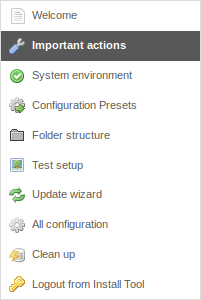
\includegraphics[width=0.7\linewidth]{Images/InstallTool/ImportantActions.png}
			\end{figure}
		\end{column}
		\begin{column}{.7\textwidth}
			\begin{figure}\vspace*{-0.4cm}
				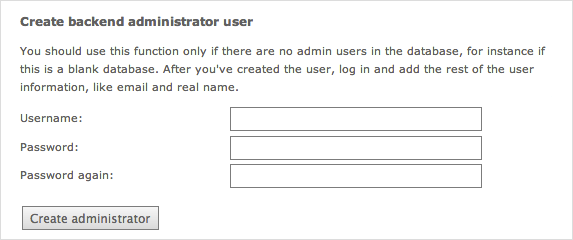
\includegraphics[width=0.9\linewidth]{Images/InstallTool/SaltedPasswords.png}
			\end{figure}
		\end{column}
	\end{columns}

\end{frame}

% ------------------------------------------------------------------------------
% Application Context
% ------------------------------------------------------------------------------

\begin{frame}[fragile]
	\frametitle{Install Tool}
	\framesubtitle{Kontekst aplikacije (1)}

	\begin{itemize}
		\item TYPO3 >= 6.2 uzima \textbf{kontekst aplikacije} u obzir\newline
			\smaller(poznato iz TYPO3 Flow)\normalsize
		\item Promenjiva okruzenja \texttt{TYPO3\_CONTEXT} postavlja kontekst\newline
			\smaller(podrazumevano: \texttt{Production}, podkontekst kao na primer \texttt{Production/Staging} je takodje moguc)\normalsize

			\begin{lstlisting}
				# File: .htaccess
				# Rules to set Application Context based on hostname:

				RewriteCond %{HTTP_HOST} ^dev\.example\.com$
				RewriteRule (.*) $1 [E=TYPO3_CONTEXT:Development]

				RewriteCond %{HTTP_HOST} ^www\.example\.com$
				RewriteRule (.*) $1 [E=TYPO3_CONTEXT:Production]

				# Sets an environment variable, which is then available to TYPO3 CMS:
				SetEnv TYPO3_CONTEXT Production
			\end{lstlisting}

	\end{itemize}

\end{frame}

% ------------------------------------------------------------------------------
% Application Context
% ------------------------------------------------------------------------------

\begin{frame}[fragile]
	\frametitle{Install Tool}
	\framesubtitle{Podrazumevana podesavanja TYPO3\_CONF\_VAR}

	\begin{columns}[T]
		\begin{column}{.5\textwidth}

			\begin{itemize}
				\item Odredjena podesavanja TYPO\_CONF\_VAR-a mogu biti definisana u Install Tool-u
				\item Podesavanja kao stop su debug output, deprecation log, devIPmask i ostali sistemski logovi, kao i nivo logovanja
				\item Ugradjeni konteksti: "Production" i "Development"\newline
					(konfiguracija po zelji korisnika je takodje moguca)
			\end{itemize}

		\end{column}
		\begin{column}{.5\textwidth}

			\begin{figure}\vspace*{-0.4cm}
				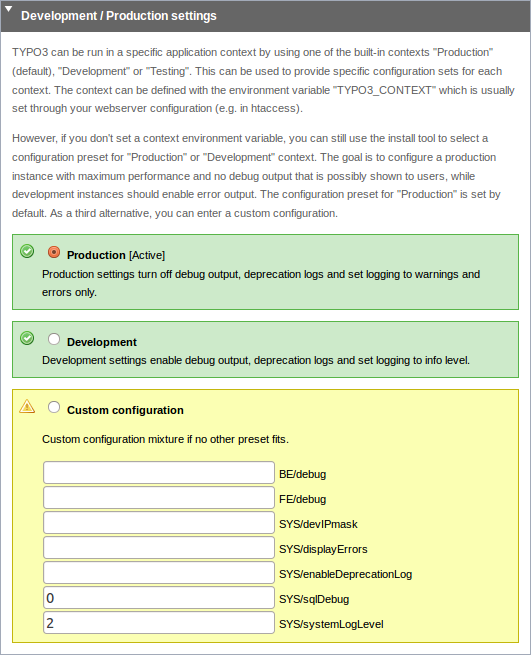
\includegraphics[width=0.8\linewidth]{Images/InstallTool/ApplicationContext.png}
			\end{figure}

		\end{column}
	\end{columns}

\end{frame}

% ------------------------------------------------------------------------------
% Improved Usability
% ------------------------------------------------------------------------------

\begin{frame}[fragile]
	\frametitle{Install Tool}
	\framesubtitle{Poboljsana upotrebljivost}

	\begin{columns}[T]
		\begin{column}{.5\textwidth}

			\begin{itemize}
				\item Fiksirana pozicija levog menija kada se skroluje 
					\begingroup\color{typo3red}\textbf{(1)}\endgroup
				\item Fiksirana pozicija dugmeta "Write configuration" na dnu
					\begingroup\color{typo3red}\textbf{(2)}\endgroup
				\item Unosi u "All Configuration" su grupisani (sekcije se otvaraju klikom na naslov) i sortirani
					\begingroup\color{typo3red}\textbf{(3)}\endgroup
			\end{itemize}

		\end{column}
		\begin{column}{.5\textwidth}

			\begin{figure}\vspace*{-0.4cm}
				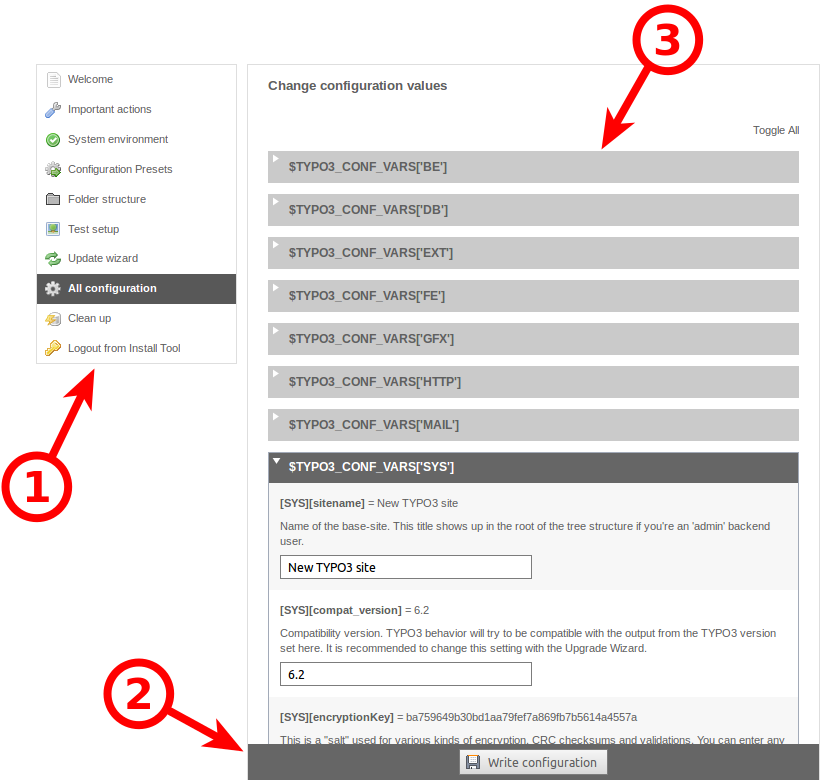
\includegraphics[width=0.8\linewidth]{Images/InstallTool/ImprovedUsability.png}
			\end{figure}

		\end{column}
	\end{columns}

\end{frame}

% ------------------------------------------------------------------------------
% Human-Friendly Error Codes
% ------------------------------------------------------------------------------

\begin{frame}[fragile]
	\frametitle{Install Tool}
	\framesubtitle{Kodovi gresaka citljivi ljudima}

	\begin{itemize}
		\item Kljucne reci sa znacenjem mogu da se koriste za sledece opcije:\newline
			(TYPO3 < 6.2: samo numericke vrednosti)
	\end{itemize}

	\begin{columns}[T]
		\begin{column}{.4\textwidth}
			\advance\leftskip+0.8cm

			\smaller
				\texttt{[SYS][errorHandlerErrors]}\newline
				\texttt{[SYS][exceptionalErrors]}\newline
				\texttt{[SYS][syslogErrorReporting]}\newline
				\texttt{[SYS][belogErrorReporting]}\newline
			\normalsize

		\end{column}
		\begin{column}{.6\textwidth}

			\begin{figure}\vspace*{-0.4cm}
				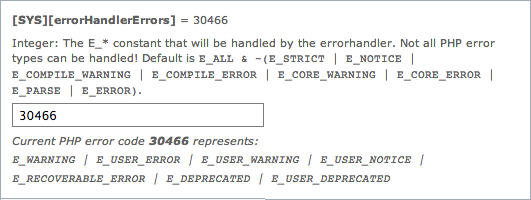
\includegraphics[width=0.9\linewidth]{Images/InstallTool/HumanFriendlyErrorCodes.png}
			\end{figure}

		\end{column}
	\end{columns}

	\vspace{0.2cm}

	\begin{itemize}
		\item Extbase ViewHelper \textbf{format.phpErrorCode} se brine za prevodjenje u PHP kodove gresaka
	\end{itemize}

\end{frame}

% ------------------------------------------------------------------------------
% Errors In Folder Structure
% ------------------------------------------------------------------------------

\begin{frame}[fragile]
	\frametitle{Install Tool}
	\framesubtitle{Greske u strukturi foldera}

	\begin{itemize}
		\item Grecke u "Folder Structure" su izlistane kao bedzevi (zaokruzen broj)
	\end{itemize}

	\begin{figure}
		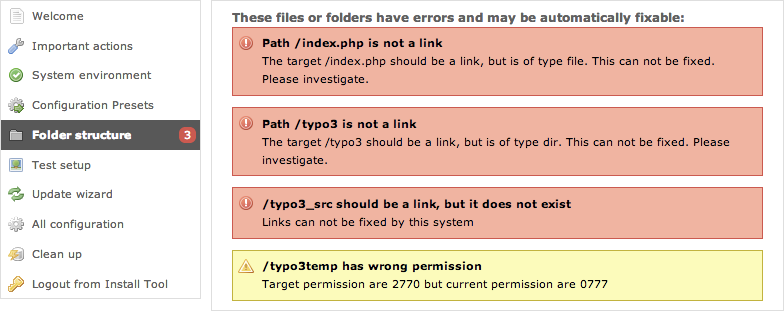
\includegraphics[width=0.95\linewidth]{Images/InstallTool/ErrorsInFolderStructure.png}
	\end{figure}

\end{frame}

% ------------------------------------------------------------------------------
% Core Updates
% ------------------------------------------------------------------------------

\begin{frame}[fragile]
	\frametitle{Install Tool}
	\framesubtitle{Core unapredjenja}

	\begin{itemize}
		\item Unapredjenje TYPO3 core-a na poslednju manju verziju sa samo jednim klikom
		\item Promenjiva okruzenja \texttt{TYPO3\_DISABLE\_CORE\_UPDATER=1} onemogucava ovu funkcionalnost
	\end{itemize}

	\begin{figure}
		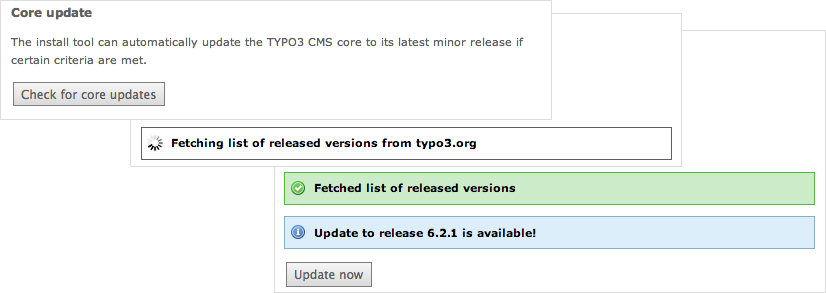
\includegraphics[width=0.95\linewidth]{Images/InstallTool/CoreUpdate.png}
	\end{figure}

\end{frame}

% ------------------------------------------------------------------------------
% Miscellaneous
% ------------------------------------------------------------------------------

\begin{frame}[fragile]
	\frametitle{Install Tool}
	\framesubtitle{Ostalo}

	\begin{itemize}
		\item Sve forme su zasticene sa CSRF (\textit{cross-site request forgery})
		\item Install Tool koristi uproscen Fluid Standalone View
		\item Samo neophodne TYPO3 funkcije se ucitavaju\newline
			(ostecen \texttt{ext\_localconf.php} ili \texttt{ext\_tables.php} ili neko prosirenje ne mogu vise da ostete Install Tool)
		\item Nova pocetna tacka:	\tabto{3.2cm} \texttt{typo3/sysext/install/Start/Install.php}\newline
			Pre:					\tabto{3.2cm} \texttt{typo3/install/index.php}\newline
									\tabto{3.2cm} (postoji redirekcija sa starog URL-a na novi)
		\item Iskljuceno kesiranje obezbedjuje da se Install Tool moze koristiti, iako kes sadrzi nevazeci PHP code
	\end{itemize}

\end{frame}

% ------------------------------------------------------------------------------
% Miscellaneous
% ------------------------------------------------------------------------------

\begin{frame}[fragile]
	\frametitle{Install Tool}
	\framesubtitle{Ostalo}

	\begin{itemize}
		\item Proverite da li PHP podesavanje \texttt{xdebug.max\_nesting\_level} pokazuje vrednost 250 ili visu (podrazumevana vrednost "100" moze da stvara probleme)
		\item "Relaxed permission check":

			\small
				Ukoliko direktorijum sajta nema ispravne permisije (na primer "2770"),
				i ovo ne moze da se resi, na primer iz razloga sto direktorijum ne pripada 
				korisniku koji je pokrenuo Install Tool, prvi korak instalacije puca.
				Opcija "targetPermissionRelaxed" smanjuje vaznost permisija i dozvoljava
				nastavak instalacije dokle god podfolderi mogu biti kreirani.
			\normalsize

	\end{itemize}

\end{frame}

% ------------------------------------------------------------------------------
% Miscellaneous
% ------------------------------------------------------------------------------

\begin{frame}[fragile]
	\frametitle{Install Tool}
	\framesubtitle{Ostalo}

	\begin{itemize}
		\item Uklonjene opcije (kljucevi) iz Install Tool-a\newline
			\small(a samim tim i iz fajla \texttt{LocalConfiguration.php}):\normalsize
	\end{itemize}

	\begin{columns}[T]
		\begin{column}{.5\textwidth}
			\advance\leftskip+0.8cm
			\smaller
				\texttt{BE/loginLabels}\newline
				\texttt{BE/loginNews}\newline
				\texttt{BE/useOnContextMenuHandler}\newline
				\texttt{EXT/em\_mirrorListURL}\newline
				\texttt{EXT/em\_wsdlURL}\newline
				\texttt{EXT/extList}\newline
				\texttt{EXT/extList\_FE}\newline
				\texttt{EXT/noEdit}\newline
			\normalsize
		\end{column}
		\begin{column}{.5\textwidth}
			\smaller
				\texttt{FE/defaultTypoScript\_editorcfg}\newline
				\texttt{FE/simulateStaticDocuments}\newline
				\texttt{GFX/noIconProc}\newline
				\texttt{GFX/TTFLocaleConv}\newline
				\texttt{SYS/additionalAllowedClassPrefixes}\newline
				\texttt{SYS/caching/cacheBackends}\newline
				\texttt{SYS/caching/cacheFrontends}\newline
				\texttt{SYS/extCache}\newline
				\texttt{SYS/T3instID}\newline
			\normalsize
		\end{column}

	\end{columns}

\end{frame}

% ------------------------------------------------------------------------------

